\section{Concept}\label{sec:concept}

In this section, we will briefly present the concept behind our implementation. We start by defining the high level requirements and continue with presenting some of our created mockups that should capture these requirements. We finish this section by explaining the assumptions on which our concept is based on.

\subsection{Requirements}\label{req}

The high-level functionality of our implementation is similar to existing car market platforms such as AutoScout24. But in contrast to AutoScout24, we will rely on blockchain technology, in our case Ethereum, to implement these use cases. However, the details of the implementation will be specified in Section~\ref{sec:impl}.

In this subsection we will lay out all the user level functionality in form of user stories. These user stories should give an intuitive overview over the desired functionality of our implementation.

\begin{enumerate}
  \item A user should be able to perform a One-Click sign-on and login by using his Ethereum account for authentication. There should be no need for using and storing additional passwords or sensible data.

  \item A logged in user should be able to list all his registered cars including information about each car such as mileage.

  \item A logged in user should be able to put one of his selected cars on sale. The sale contains among other information the price and can be enriched by further details such as images of the car or a description.

  \item Any user should be able to search for offered cars. By providing search filters, the user should be able to limit the search results to a list of cars that meets his requirements.

  \item If an user decides to buy a car on sale, he should be able to contact the seller by email beforehand.

  \item A logged in user should be able to buy a car by paying the requested price.

  \item The car transfer from the seller to the buyer should automatically be performed, as well as the money transfer from the buyer to the seller.

\end{enumerate}

\subsection{Mockups}

Before implementing our requirements, formulated in the previous subsection, we designed some screen mockups in order to understand how the user interface should look like. For that, we used \textit{Balsamiq}~\cite{Balsamiq}.

In Figure \ref{fig:mockup_01} and Figure \ref{fig:mockup_02} two exemplary mockups are shown, displaying one specific screen respectively. The first one displays the home screen, while the latter one displays the search result screen. It is worth mentioning that we did not implement every button or text field displayed in the mockup screens. Instead, we used these mockups as a rough guideline for the implementation process and as discussion ground for early design decisions.

\begin{figure}[htbp]
\centerline{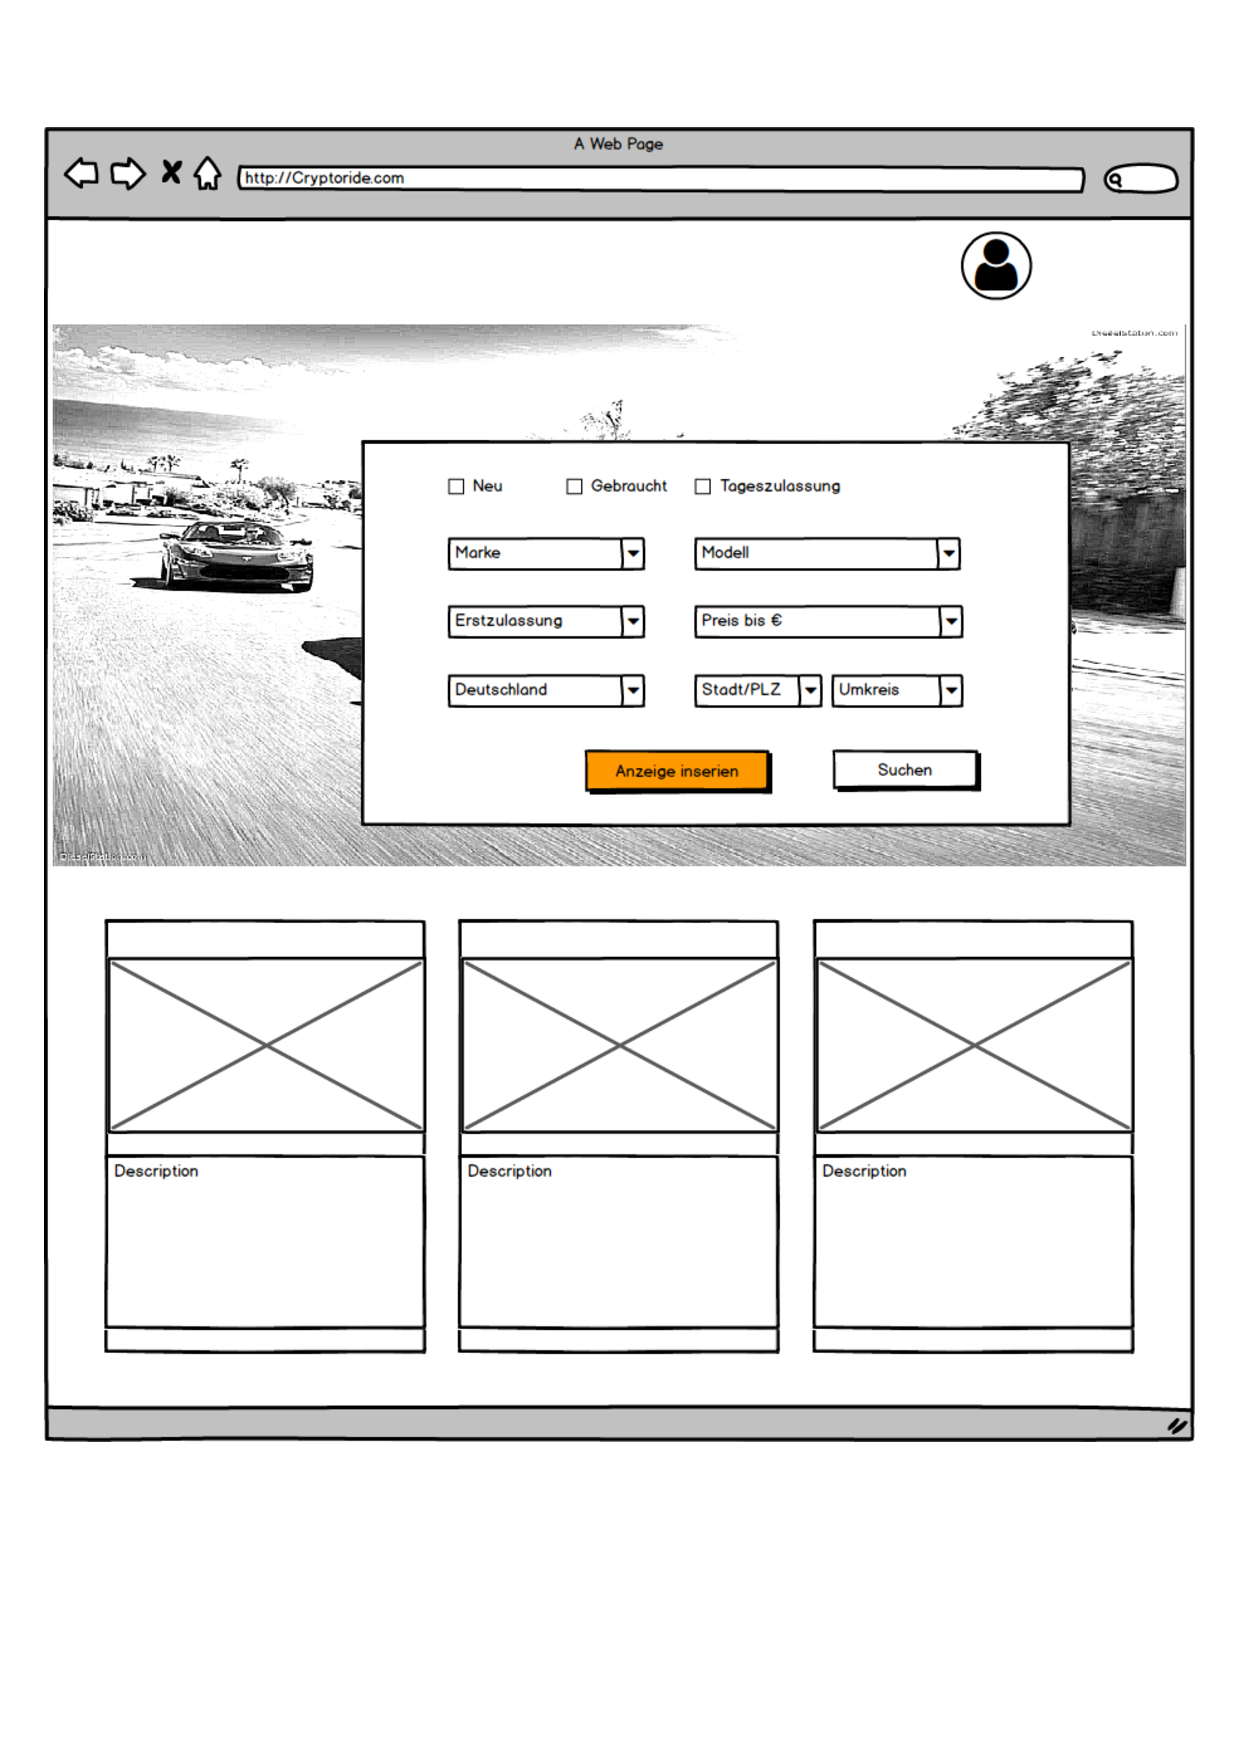
\includegraphics[width=0.9\textwidth]{figures/mockup_screen_01.pdf}}
\caption{Mockup of the home screen \label{fig:mockup_01}}
\end{figure}

\begin{figure}[htbp]
\centerline{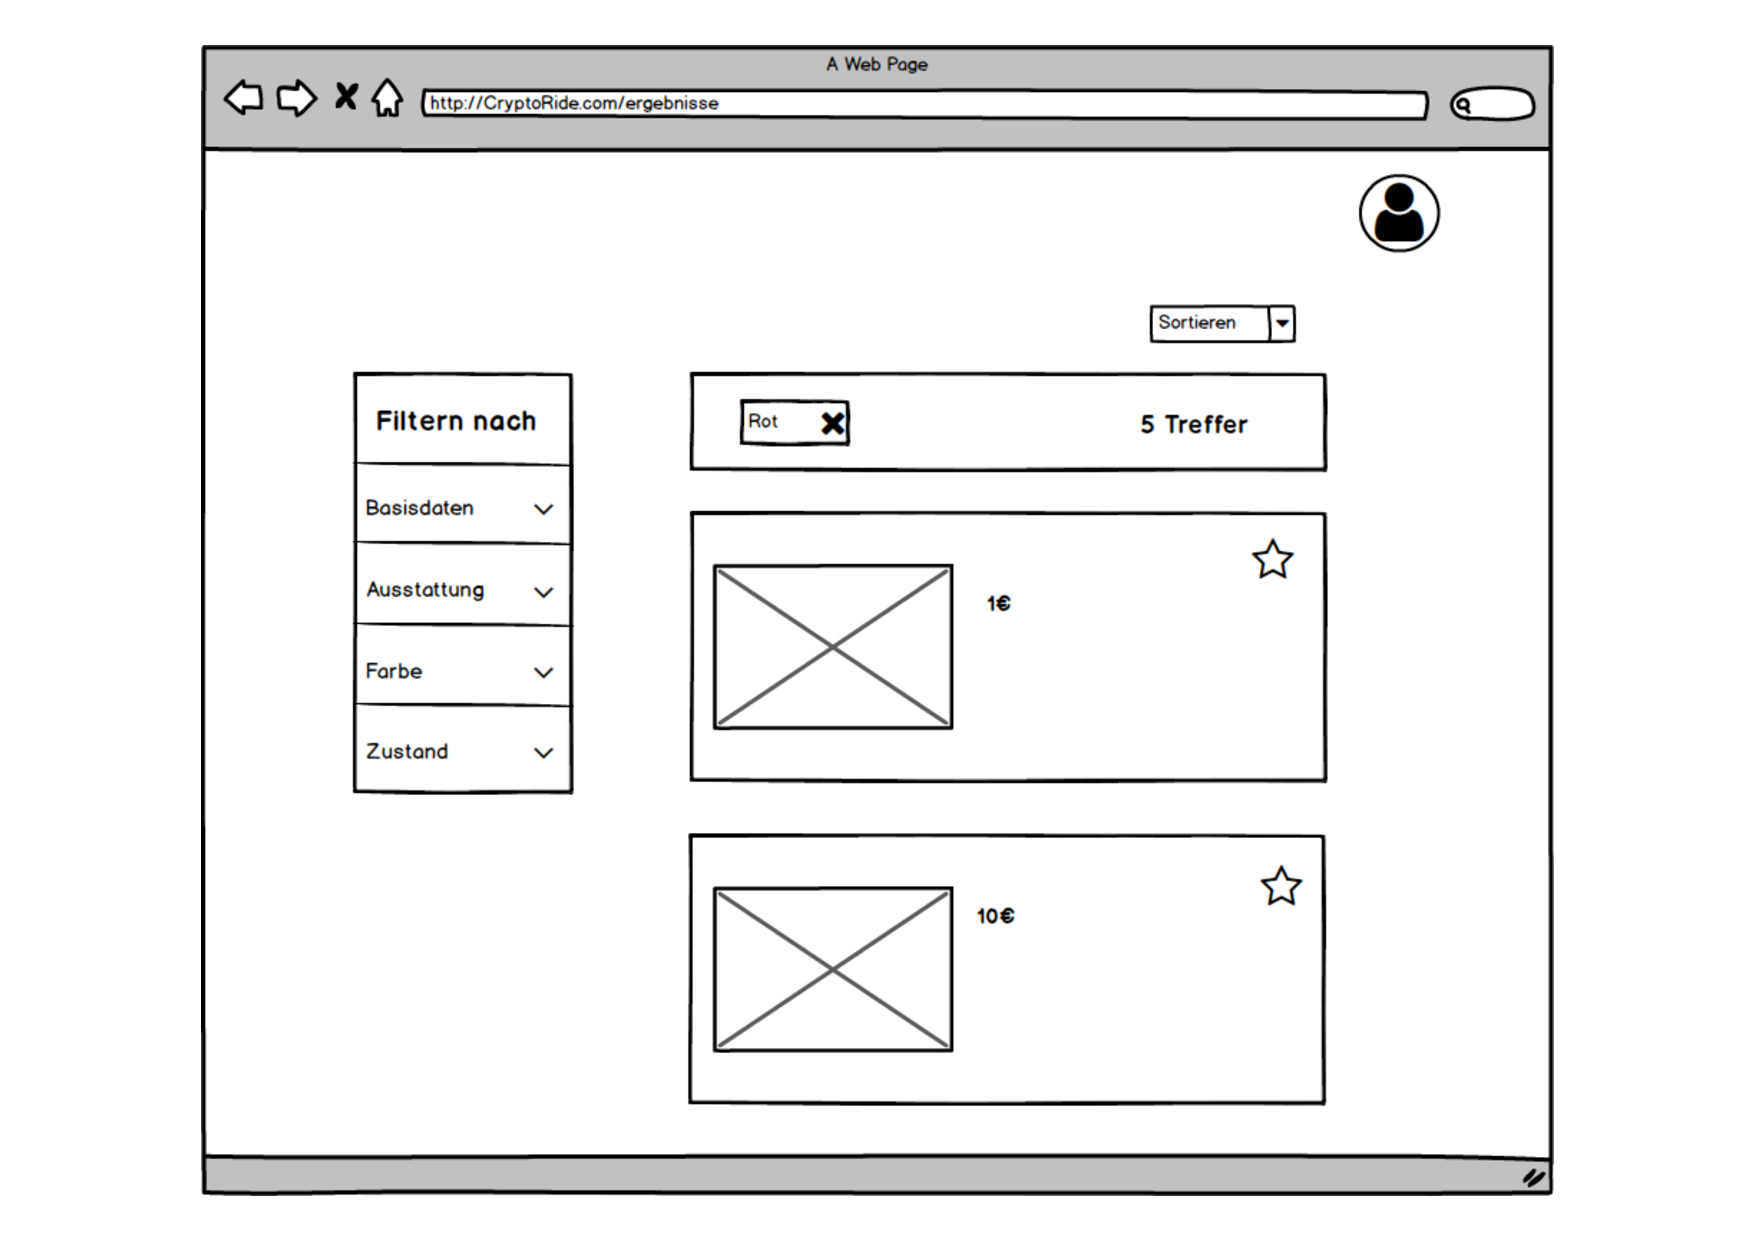
\includegraphics[width=0.9\textwidth]{figures/mockup_screen_02.pdf}}
\caption{Mockup of the search result screen \label{fig:mockup_02}}
\end{figure}


\subsection{Assumptions}\label{concept:assumptions}

Our approach is based on some assumptions regarding the car ecosystem. This includes car manufacturing, as well as compliance visits and mileage logging. At the current state, our approach would not be possible to implement in a way that it could provide the desired advantages mentioned in Section~\ref{sec:selling_points}. However, we do believe that adoption of blockchain technologies will eventually rise over the upcoming years.

Therefore, we assume in our scenario that car manufacturers already leverage blockchain technology. In specific, we make the following two assumptions. Firstly, when a car manufacturer produces a new car, it stores the car's identity on a blockchain which can be accessed by third-parties on demand. However, only car manufacturers are able to create a car on the blockchain. Secondly, we assume that new cars will be built in a way that enables them to store and update, on a regular basis, some of their key information, such as mileage, on a blockchain. Alternatively or additionally to the second point, we assume that trusted third-parties would be allowed to update details of a car, e.g the number of accidents, on the blockchain.
